\documentclass[11pt]{article}

\usepackage[utf8]{inputenc}
\usepackage[T1]{fontenc}

\usepackage[a4paper, left=2cm, right=2cm, top=3.5cm, bottom=3.5cm]{geometry}
\usepackage[french]{babel}

% Paragraph spacing
\setlength{\parskip}{1em}

% Fancy headers
\usepackage{fancyhdr}

% Captions for subfigures
\usepackage{subcaption}

% Code highlighting
\usepackage{minted}

% Footnote inside a caption
\usepackage{fnpos}
\usepackage{ftnxtra}

% Maths
\usepackage{amsmath}
\usepackage{amssymb}

% Todo notes
\usepackage{todonotes}

% Table of contents for bibliography
\usepackage[nottoc]{tocbibind}

% Inline monospace font
\def\code#1{\texttt{#1}}

% Figures
\usepackage{graphicx}

% Draw figures
\usepackage{tikz}

% Tikz node rotation
\usetikzlibrary{positioning}

% Turing machine
\usetikzlibrary{chains,fit,shapes}

% Usage: \rotnode[options]{rotation}{text}
\newcommand\rotnode[3][]{%
    \node [#1, opacity=0.0] (tmp) {#3};
    \node [draw, rotate around={#2:(tmp.center)}] at (tmp) {#3};
}

% Clickable links
\usepackage{hyperref}

% Table of contents depth
\setcounter{tocdepth}{2}

% Inline code
\usepackage{listings}
\usepackage{color}

\title{Systèmes d'exploitation : processus}

\author{William SCHMITT}
\date{2018-2019}

\begin{document}
\maketitle

\section{Problème}

A l'époque où la mémoire était plus rapide que les processus, on a eu l'idée de rajouter plusieurs unités de calcul.

\begin{figure}[ht]
    \centering
    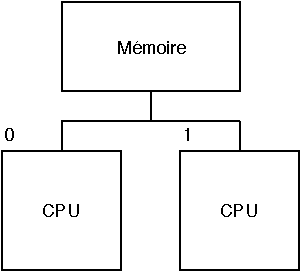
\includegraphics{img/c4-multicpu.pdf}
\end{figure}

Exemple de code assembleur exécuté sur deux CPU en parallèle.
\begin{minted}[frame=single]{asm}
    ; début section critique
    load $i, %r0
    inc %r0
    store %r0, $i
    ; fin section critique
\end{minted}

Quel est le résultat stocké dans i ?

Selon l'ordre des opérations, on peut obtenir 1 ou 2.
Intervient alors l'algorithme de Dekker (1966), permettant de garantir l'obtention du résultat souhaité : 2.

\section{Solutions}
\setcounter{subsection}{-1}

\subsection{Booléens et sections critiques}
Une première idée est de définir des sections critiques à l'aide de booléens.

\begin{minted}[frame=single]{c}
    bool occ = false;
    debut_sc() {
        alpha:  if (occ)
                    goto alpha;
                occ = true;
    }

    fin_sc() {
        occ = false;
    }
\end{minted}

Ce code est faux car on n'a pas d'exclusion mutuelle.

\subsection{Ecriture de \mintinline{c}{occ} avant le test}
\begin{minted}[frame=single]{c}
    bool occ = false;
    debut_sc() {
        bool old = occ
        occ = true;
        alpha:  if (occ)
                    old = occ;
                    goto alpha;
    }

    fin_sc() {
        old = false
    }
\end{minted}

Cela ne résoud pas le problème, puisque la variable old est locale et en cas de lancement simultané, on se ramène au même cas de figure que précédemment.

\subsection{Tickets}

Il faut ici connaître son numéro de processeur, à cet effet on considère avoir à disposition un registre \mintinline{c}{p} permettant de récupérer son numéro de processeur. On peut donc calculer \mintinline{c}{q = (1-p)}, le numéro de l'autre processeur.
\begin{minted}[frame=single]{c}
    int tour = 0;
    debut_sc() {
        alpha:  if (p != tour)
                    goto alpha;
    }

    fin_sc() {
        tour = q
    }
\end{minted}

L'exclusion mutuelle fonctionne bel et bien, mais si l'un des deux processus souhaite exécuter la section critique mais que l'autre ne l'exécute pas, le premier sera sujet à de la \textbf{famine} : il attendra pour toujours.

\subsection{Tableaux}
On continue à utiliser le registre \mintinline{c}{p}. Cette fois-ci chaque CPU peut annoncer sa demande avant la boucle.
\begin{minted}[frame=single]{c}
    bool acces[2] = { false }
    debut_sc() {
        acces[p] = true
        alpha:  if (acces[q])
                    goto alpha;
    }

    fin_sc() {
        acces[p] = false
    }
\end{minted}

L'exclusion mutuelle est vérifiée, mais il y a un risque de boucle infinie en cas d'exécution simultanée : c'est un \textbf{dead-lock} (ou \textbf{interblocage}). 

\subsection{Tableaux 2 : electric boogaloo}

On garde le principe de la solution précédente avec un renoncement à une demande et en recommençant.

\begin{minted}[frame=single]{c}    
    bool acces[2] = { false, false }
    debut_sc() {
        alpha:  acces[p] = true;
                if (acces[q])
                        acces[p] = false;
                            
                    goto alpha;
    }

    fin_sc() {
        acces[p] = false
    }
\end{minted}

On observe un interblocage si l'exécution est synchrone, qu'on peut donc résoudre ainsi :

\begin{minted}[frame=single]{c}    
    bool acces[2] = { false, false }
    debut_sc() {
        alpha:  acces[p] = true;
                if (acces[q])
                        acces[p] = false;
                        sleep(random(delta)) // avec "recursive doubling" : 1 2 4 8 ...
                    goto alpha;
    }

    fin_sc() {
        acces[p] = false
    }
\end{minted}

On peut initialiser la graine de la fonction random par le numéro du CPU (par exemple).

\subsection{Tour + tableaux + renoncement}
Celui dont ça n'est pas le tour renonce.

\begin{minted}[frame=single]{c}    
    bool acces[2] = { false }
    int tour = 0;
    debut_sc() {
        alpha:  acces[p] = true;
                if (access[q])
                    if (tour != p)
                        acces[p] = false;
                        goto alpha;
    }

    fin_sc() {
        tour = q;
        acces[p] = false
    }
\end{minted}

Il n'y a pas d'exclusion mutuelle cas la condition \mintinline{c}{access[q]} est fausse, donc on ne boucle pas.

\subsection{Algorithme de Dekker}
\begin{minted}[frame=single]{c}    
    bool acces[2] = { false }
    int tour = 0;
    debut_sc() {
        alpha:  acces[p] = true;
                if (access[q])
                    if (tour == p) {
                        beta:   if (acces[q])
                                    goto beta;
                    }
                    else
                    {
                        acces[p] = false;
                        gamma:  if (tour == q)
                                    goto gamma;
                                goto alpha
                    }
    }

    fin_sc() {
        tour = q;
        acces[p] = false
    }
\end{minted}

On ne demande pas son accès tant que ça n'est pas son tour.

\subsection{Algorithme de Petersen}
15 ans plus tard, Petersen propose cette solution bien plus simple.

\begin{minted}[frame=single]{c}    
    bool acces[2];
    int dernier;
    debut_sc() {
        acces[p] = true;
        dernier = p;
        alpha:  if (acces[q])
                    if (dernier == p)
                        goto alpha;
    }

    fin_sc() {
        acces[p] = false;
    }
\end{minted}

On se sert de la variable \mintinline{c}{dernier} pour savoir lequel attend (qui est donc le dernier à avoir écrit dans la variable).
\end{document}